\documentclass{report}
\usepackage{fullpage}
\usepackage{amsmath}
\usepackage{graphicx}
\renewcommand{\baselinestretch}{2}
\author{Saran S - 133106001 \\ Rahul Joshi - 133106002 \\ Department of Mechanical Engineering \\ IIT Bombay}
\title{ME 766 Project report \\ Parallelization of Advection Schemes using MPI}
\begin{document}
\maketitle
\section*{Problem Definition}
A 2D Cartesian $(x,y)$ computational domain of size $L=1m$ and $H=1m$, for computational heat advection of a fluid ($\rho=1000\frac{Kg}{m^3}$ and $C_p=4180\frac{W}{mK}$) moving with a uniform velocity $u=v=1\frac{m}{s}$ and an initial temperature of 50C. The left and top boundary of the domain is subjected to 100C and the bottom and right boundary to 0C. Using the physics based finite volume solution methodology, developed a computer program for the above problem, and ran the code for First Order Upwind scheme(FOU). We varied the maximum number of grid points in x-and y-direction in the range of 102 to 1002 and convergence criteria as 20000 iterations. Figure \ref{fig:schematic} shows the schematic of the problem discussed above.
\begin{figure}[h]
\centering
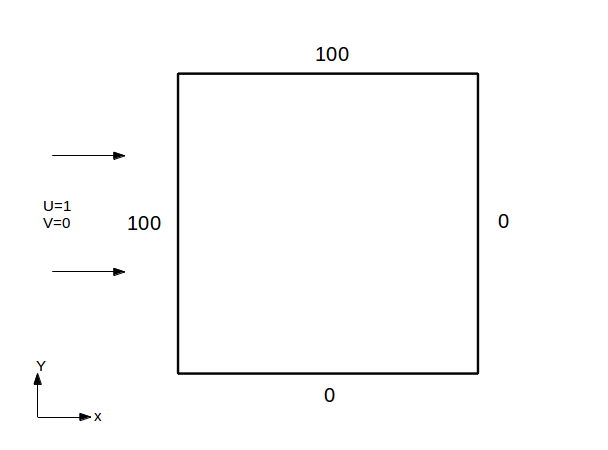
\includegraphics[width=0.5\textwidth]{1}
\caption{Schematic of problem}
\label{fig:schematic}
\end{figure}

\section*{Implementation method}
Initially a serial vectorized code for the above discussed problem was implemented on Python platform using Numpy module, which is specific for scientific computations. Non-vectorized code works on a single pair of operands at a time, where as vectorized code works on multiple pair of operands and optimize the code for better performance. So vectorization could be considered as an implicit parallelism done by the vectorising compiler available in the modern computers. 

\end{document}